\chapter[Quantum Relational Dynamics for Interacting Quantum Systems]{Relational Quantum Mechanics: With System and Environment Interaction\label{chap:sebgem_Rel}}

We start our realtional description, by \emph{reformulating} the time independent Schr\"odinger equation as an \emph{invariance principle}~\cite{Gemsheim:2023izg}
\begin{equation}
    \label{eq:invariance_principle}
        \exp\left[i\lambda(\H - E\I)\right] \ketPsi = \ketPsi. 
\end{equation}
Where  \(\lambda\) is any complex-valued parameter, $\H$ is the Hamiltonian of the global system, and \(\ketPsi\) is the global state vector. Differentiating (\refeq{eq:invariance_principle}) with respect to \(\lambda\) one gets  the usual Time Independent Schr\"odinger Equation (TISE)
\begin{equation*}
    \H \ketPsi = E \ketPsi.
\end{equation*}

For our analysis, we assume that \(\lambda\) is real. There is no fundamental reason on why \(\lambda\)
should be real. However, assumption of realness of \(\lambda\) is a phenomological observation, 
based on the fact that the time evolution operator is unitary operator for a
closed quantum system. The unitarity of the time evolution operator and  the hermiticity of the Hamiltonian
implies that the parameter \(\lambda\) has to to real. 


We partition the total Hilbert space $\mathcal{H}$ into two components to extract the dynamics. A system \(\mathcal{H}_s\) and a clock \(\mathcal{H}_c\). We re-write 
\begin{equation}
    \H = \H_s \otimes \I_c + \I_s \otimes \H_c + \Vinter .
\end{equation}

Since the system and environment\footnote{Please note that the words `clock' and `environment' will be used synonymous. The term ``system" denotes a subsystem (excluding the environment) of a global Hilbert space unless otherwise specified.} are embedded in the global Hilbert space, one can single
out the system state by projecting the global state partially onto a static state of the environment. 

\paragraph{For non-interacting system and environment:} Let \(\ket{\chi}\) be a state vector 
in clock Hilbert space. 

We choose some state \(\ket{\chi_0} \in \mathcal{H}_c\). If one projects the state vector \(\ket{\chi_0}\) onto the invariance equation~(\refeq{eq:invariance_principle}) (assuming the absence of interaction, represented by \(\Vinter = \oper{0})\), one gets
\begin{equation}
\begin{gathered}
\bra{\chi_0}e^{i\lambda(\H - E)}\ketPsi = \innerGlob{\chi_0}{\Psi}\\
\bra{\chi_0}e^{i\lambda(\H_c - E)}\ketPsi =e^{-i\lambda \H_s}  \innerGlob{\chi_0}{\Psi}.
\end{gathered}
\end{equation}
We define
\begin{equation}
   \ket{\chi_\lambda} = e^{-i\lambda(\H_c - E)}\ket{\chi_0}.
\end{equation}

By conditioning the global state \(\ketPsi\) onto a clock state \(\ket{\chi_\lambda}\),
we utilize the state \(\ket{\chi_\lambda}\) as a label to associate the system state with the particular value of \(\lambda\), i.e., 
\begin{equation}
    \label{eq:nonint_sys_evol}
    \ket{\varphi(\lambda)}_s \equiv \innerGlob{\chi_\lambda}{\Psi}.
\end{equation}
So, 
\begin{equation}
\label{eq:nonint_sys_evol}
    \ket{\varphi(\lambda)}_s = e^{-i\lambda \H_s} \innerGlob{\chi_0}{\Psi} \equiv e^{-i\lambda \H_s}\ket{\varphi(0)}_s.
\end{equation}

Notice that the choice of \(\ket{\chi_0}\) fixes the system's initial state.
Since, \(\lambda\) in (\refeq{eq:nonint_sys_evol}) is assumed to be a continuous 
 parameter, the above equation can be interpreted as a solution to the differential equation
\begin{equation}
    i \dfrac{d}{d\lambda} \ket{\varphi(\lambda)}_s = \H_s \ket{\varphi(\lambda)}_s.
\end{equation}
Which is equivalent to (Time-dependent Schr\"odinger Equation) TDSE in units 
\(\hbar = 1\). It is crucial for the system and the environment within the global Hilbert space to exhibit entanglement. Otherwise, the system and the environment would uphold separate ``global" invariance principles, each with its own parameter, \(\lambda_s\) and \(\lambda_c\), respectively. This would leave the relationship between \(\lambda_s\) and \(\lambda_c\) unresolved~\cite{Gemsheim:2023izg}.

\paragraph{Role of parameter \(\lambda\):} The variable \(\lambda\) introduced 
in the above derivation has no physical significance. It only serves as a parameter
to track the evolution of our system. Any reparametrization of \(\lambda \to t(\lambda)\) 
has no change in the equation of the system state evolution, highlighting
the time reparametrization invariance of the global system. One can, in principle 
\footnote{As one does it always. We never measure time directly; rather, we measure
the angular position of a clock dial or the no of transition electrons made in a cesium atom.}
 parameterize the evolution using an observable of our environment 
 \(\operatorname{A}_c(\lambda)\equiv \bra{\chi_\lambda}\oper{A}_c\ket{\chi_\lambda}\). 
 An ideal choice would be to use such a $\oper{A}_c$ for which the relation between $\lambda $ and $\operatorname{A}_c$ is simple, for example, linear.

High-resolution clock states $\ket{\chi_\lambda} \propto \sum_k a_k \exp (-i\lambda E_c ^k)\ket{E_c}_k$ require a broad 
distribution over the clock energy eigenstates, ideally with uniform coefficients 
($a_k$)~\cite{Gemsheim:2023izg, Smith:2017pwx}. This condition is readily met when the clock's physical dimensions exceed those of the system.


\paragraph{For interacting system and environment:} So far in our analysis, we have assumed 
no interaction, i.e., \(\Vinter = \oper{0}\). However, in real scenarios, one always has some
interaction within components of a global closed system. To extend the derivation to 
non-zero \(\Vinter\), we modify our clock state as
\begin{equation}
   \begin{gathered}
      \ket{\chi_\lambda} = e^{-i\lambda(\H_c - E)}\ket{\chi_0} \to \\\ket{\chi_\lambda}
       = e^{-iS(\lambda)}e^{-i\lambda(\H_c - E)}\ket{\chi_0}
   \end{gathered}
\end{equation}
where \(S(\lambda) = \int^{\lambda}\xi(\tilde{\lambda} ) d\tilde{\lambda}\) is an extra factor introduced for 
simplifying upcoming derivations. When  projected onto this, the global state can be written as
\begin{equation}
\label{eq:TISE_undecomposed}
    \left(-\H_s + \xi(\lambda) + i\dfrac{d}{d\lambda}\right) 
    \innerGlob{\chi_\lambda}{\Psi} = \bra{\chi_\lambda}\Vinter\ketPsi.
\end{equation}
We can rearrange the above equation to write it as
\begin{equation}
\label{eq:TISE_undecomposed_simp}
    \begin{gathered}
         i\dfrac{d}{d\lambda}\innerGlob{\chi_\lambda}{\Psi} =
          \H_s\innerGlob{\chi_\lambda}{\Psi} - \xi(\lambda)\innerGlob{\chi_\lambda}{\Psi}  + \bra{\chi_\lambda}\Vinter\ketPsi.
    \end{gathered}
\end{equation}

We now decompose $\bra{\chi_\lambda}\Vinter\ketPsi$ into a Hermitian potential and a c-number. To facilitate the decomposition, we define the following:
 \begin{equation}
     \begin{gathered}
         \oper{P}_\Psi =\kket{\Psi} \bbra{\Psi}, \quad \oper{P}_\chi = \I_s \otimes \ket{\chi_\lambda}\bra{\chi_\lambda}\\
         \oper{P}_{\Psi \chi} = \oper{P}_\Psi\oper{P}_\chi /\mathcal{N}_\lambda
     \end{gathered}
 \end{equation}
where \(\mathcal{N}_\lambda = \bbra{\Psi}\oper{P}_\chi\ketPsi\). One observes that
\begin{equation}
\oper{P}_{\Psi \chi}\ketPsi = \frac{\oper{P}_\Psi\oper{P}_\chi}{\mathcal{N}_\lambda} \ketPsi
    = \ketPsi
\end{equation}
 Using above defined operators, we decompose the 
 \begin{equation}
 \label{eq:effective_Vs}
     \begin{aligned}
         \bra{\chi_\lambda}\Vinter\ketPsi = \bra{\chi_\lambda}\Vinter\oper{P}_{\Psi \chi}\ketPsi\\
         = \left[\oper{V}_s (\lambda)- \bbra{\Psi} \oper{V}\oper{P}_\chi \ketPsi/\mathcal{N}_\lambda \right] \innerGlob{\chi_\lambda}{\Psi}
     \end{aligned}
 \end{equation}
where 
\begin{mdframed}
    \begin{equation}
        \label{eq:chap3_effective_Vs}
        \Vs(\lambda) = \frac{\bra{\chi_\lambda} \left(\Vinter\oper{P}_{\Psi} + \oper{P}_{\Psi}\Vinter\right)\ket{\chi_\lambda}}{\mathcal{N}_\lambda}
    \end{equation}
\end{mdframed}

Inserting (\refeq{eq:effective_Vs}) into (\refeq{eq:TISE_undecomposed_simp}) and setting \(\xi(\lambda) = -\bbra{\Psi} \oper{V}\oper{P}_\chi \ketPsi/\mathcal{N}_\lambda\) we obtain
\begin{mdframed}
    \begin{equation}
        \label{eq:chap3_sebgem_TDSE}
         { i\dfrac{d}{d\lambda}\ket{\varphi(\lambda)}_s= \left[\H_s + \Vs (\lambda)\right]\ket{\varphi(\lambda)}_s},
        \end{equation}
\end{mdframed}
where we defined \(\innerGlob{\chi_\lambda}{\Psi} = \ket{\varphi(\lambda)}_s\).  The phase factor  \(S(\lambda) = \int^\lambda \xi(\tau)d\tau \) introduced helps eliminate the c-number after the decomposition of the ``effective'' potential. 

We find that the final form of the Equation is equivalent to the TDSE for the remaining sub-system (\(\mathcal{H}_s\)) of the
global Hilbert space \(\mathcal{H}\).

\section{Example: Dynamics of two interacting two level system\label{sec:chap3_2spin_interact}}

To provide an illustrative example of the approach, let us consider an interaction two spin-1/2 particles~\cite{Gemsheim:2023izg}.
The Hamiltonians for system and clock are taken as, \(\oper{H_s} = 0\), \(\oper{H_C} = E_C\oper{\sigma}_{C, x}\)
and the interaction 
\(\Vinter = V_0\left(\oper{\sigma}_{S, x} + \oper{\sigma}_{S, z}\right)\otimes \oper{\sigma}_{C, x}\). 
Taking \(E_C = V_0 \equiv 1\), we get
\begin{equation}
    \H = \begin{pmatrix}
        1 & 1 & 0 & 1 \\
        1 & -1 & 1 & 0 \\
        0 & 1 & 1 & -1 \\
        1 & 0 & -1 & -1
        \end{pmatrix}
\end{equation}
with eigenvalues \(E = \left\{-\sqrt{3}, \sqrt{3}\right\}\), 
where both of them are doubly degenerate. One of the eigenvector
corresponding to \(E_- = -\sqrt{3}\), in the standard basis, is
\(\vec{\Psi} = \left(1, 0, -1, -(1 + \sqrt{3})\right)^T\)[refer to ~\refapp{app:chap3_appendix} for detailed calculations].
\begin{figure}[!h]
    \centering
    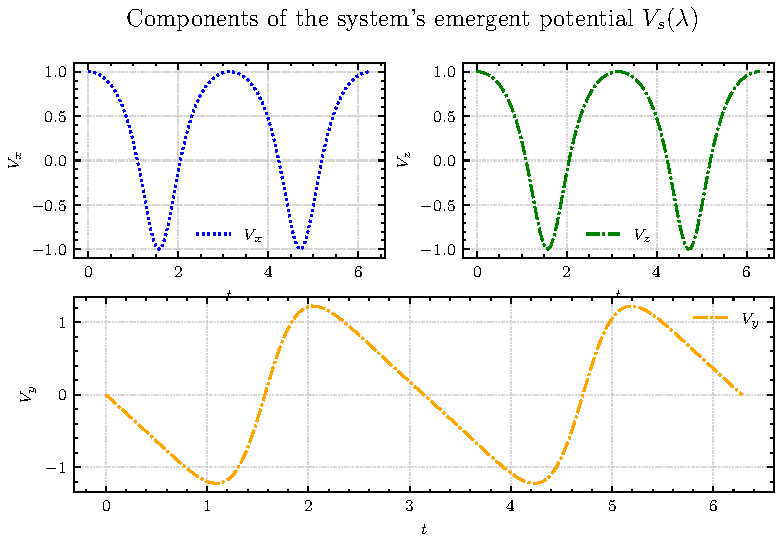
\includegraphics[width=1.0\textwidth]{chap3/Vx_Vy_Vz.pdf}
    \caption{Components of the effective potential \(\vec{V}_S(\lambda)\) for the two interacting spin-1/2 particles.}
    \label{fig:chap3_effective_potential}
\end{figure}


Taking
\begin{equation}
    \ket*{\chi(\lambda)} = 
    \frac{\exp\left(i E_- \lambda\right)}{
        2\sqrt{1 + a \cos^2(\lambda)}} \left(e^{-i\lambda} \ket*{\uparrow} + e^{i\lambda} \ket*{\downarrow} \right)
\end{equation} 
where \(a = \sqrt{3} + 1\), we obtain from \refeq{eq:effective_Vs}, the effective potential

\begin{equation}
    \oper{V}_s = \vec{V}_S(\lambda)\cdot\vec{\oper{\sigma}}_S. 
\end{equation}

\begin{figure}[!h]
    \centering
    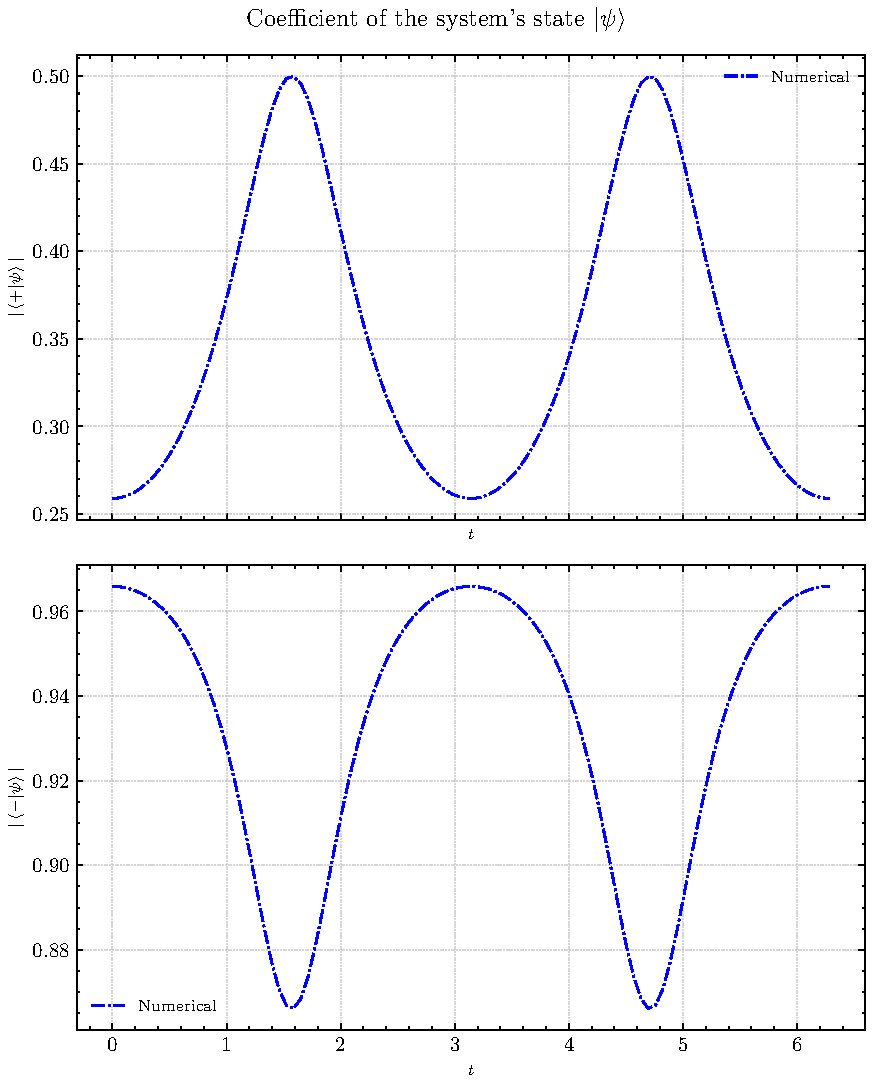
\includegraphics[]{chap3/psi_c1_c2.pdf}
    \caption{Evolution of the system state \(\ket{\varphi(\lambda)}_s\) for the two interacting spin-1/2 particles. }
    \label{fig:2spin_interact_RQM}
\end{figure}

The components of \(\vec{V}_S(\lambda)\) are shown in \reffig{fig:chap3_effective_potential} and 
are explicitly given by 
\begin{equation}
    \begin{gathered}
        V_x(\lambda) = V_z(\lambda) = \frac{\cos(2\lambda) + a \cos^2(\lambda)}{1 + a\cos^(\lambda)}\\
        V_y(\lambda) = -\frac{(a/2)\sin(2\lambda)}{1 + a \cos^2(\lambda)}
    \end{gathered}
\end{equation}



One can calculate the evolution of the system state by projecting the global state onto the clock state,
which gives
\begin{equation}
    \begin{gathered}
        \ket{\varphi(\lambda)}_s \equiv  \innerGlob{\chi(\lambda)}{\Psi} 
        = \frac{\exp\left(i a\lambda\right)}{
            2\sqrt{1 + a \cos^2(\lambda)}} \left[\ket*{\uparrow} - 
            \left(a e^{-2i\lambda} + 1\right)\ket*{\downarrow}\right] .
    \end{gathered}
\end{equation}
The dynamics is shown in \reffig{fig:2spin_interact_RQM}. 
One of the features of utilizing the relational approach is that, 
it enables us to obtain analytical solutions for the evolution of system states, even in the presence of complex time-dependent potentials that pose challenges for conventional methods. Consequently, the relational approach not only lends significance to the time parameter but also offers a viable means to address the dynamics of systems subject to arbitrary time-dependent potentials.



\newpage